\documentclass[10pt,a4paper]{article}
\usepackage[utf8]{inputenc}
\usepackage{amsmath}
\usepackage{amsfonts}
\usepackage{amssymb}
\usepackage{graphicx}
\usepackage{rotating}

\usepackage{hyperref}
\hypersetup{
	colorlinks,
	citecolor=black,
	filecolor=black,
	linkcolor=black,
	urlcolor=black
}

\author{Ben Miller}
\title{CSE321 Project 2}
\begin{document}
	\maketitle
	\pagebreak
	\tableofcontents
	\pagebreak
	\section{Specifications}
	This is the documentation for a simple security system. It will lock or unlock based off of a four digit pass code, which for the purposes of this assignment will be 9407. The combination will be entered via a 4x4 matrix keypad. Two LEDs will act as the output, lighting up depending on the validity of an input combination. A third LED will light up upon each properly processed input. Additionally, an attached LCD display will show whether the system is currently locked or unlocked.
	\pagebreak
	\section{Features}
	As previously mentioned, this will be a security system that checks for an input combination of 9407. Depending on the correctness of the user's input, the system will display difference pieces of information.
	
	The system has four states it will ultimately check for.
	\begin{itemize}
		\item An incorrect input with a locked system.
		\item An incorrect input with an unlocked system.
		\item A correct input with a locked system.
		\item A correct input with an unlocked system.
	\end{itemize}
	There is also a fifth state which will reset the current input; this will be described in further detail below. 
	
	Below is how the system would react when presented with one of the above scenarios.
	\begin{enumerate}
		\item An incorrect input with a locked system.
		\begin{itemize}
			\item Nothing happens, with the system remaining locked. The LCD will still display a locked mode and the red LED will remain lit, informing the user their last input was invalid.
		\end{itemize}
		\item An incorrect input with an unlocked system. 
		\begin{itemize}
			\item The system will lock. This will allow easy locking of the system by the user; they can simply input a random series of numbers. The LCD will change its display from unlocked to locked and the red LED will light up.
		\end{itemize}
		\item A correct input with a locked system.
		\begin{itemize}
			\item Of course, should a correct input be provided to a currently locked system, the system will unlock. The LCD will change from locked to unlocked, and the blue LED will light up, informing the user of a correct input.
		\end{itemize}
		\item A correct input with an unlocked system.
		\begin{itemize}
			\item Similarly to the first state, should a correct input be given to an unlocked system nothing will happen. The system will remain unlocked, with the LCD maintaining its display and the blue LED remaining lit.
		\end{itemize}
	\end{enumerate}
	It was described above that there was a fifth state that will act as a ``password reset.'' This is true, and will be recognized by the system via the `A' key on the keypad. Should at any moment this button get pressed, the system will clear its memory. The current LED will remain lit (i.e. if the last input was incorrect, the red LED will remain on), and the LCD will not change its display. This can occur at any point, regardless of how many values had previously been sent. 
	
	It should be noted that the numerical values 0-9 and `A' are the only recognized inputs. Pressing any of the following keys will do nothing: `B', `C', `D', `*', and/or `\#'. For any input, including the listed invalid inputs here, a green LED will briefly (for approximately 500 microseconds) light up informing the user the system received an input, whether it be valid or invalid.
	
	Lastly, the system can, provided power, run indefinitely.
	\pagebreak
	\section{Applications}
	While the applications of such a simplistic security system are admittedly limited, there are some realistic usages that can be considered. A simple system such as this one can be used for minimalistic security clearance at public facilities (e.g. a supermarket). 
	
	Given the uncomplicated implementation of the design, it can additionally be expanded upon quite easily. Changing the four-digit pass-code to an eight-digit one would be relatively straightforward, and more advanced hardware could allow for more than just the five previously described states. More advanced hardware, such as a better LCD display in conjunction with a more powerful central system, could allow multiple passwords and users to be associated with them.
	
	In summary, in its current state the industrial and retail applications of such a system are too limited to be of practical use; it can be brute forced due to its lack of a input cool-down, ignoring the abundantly obvious fact that such rudimentary hardware could simply be ignored. However, this simplicity is arguably an advantage, allowing for a large amount of room for expansion and improvement.
	\pagebreak
	\section{Block Diagram}
	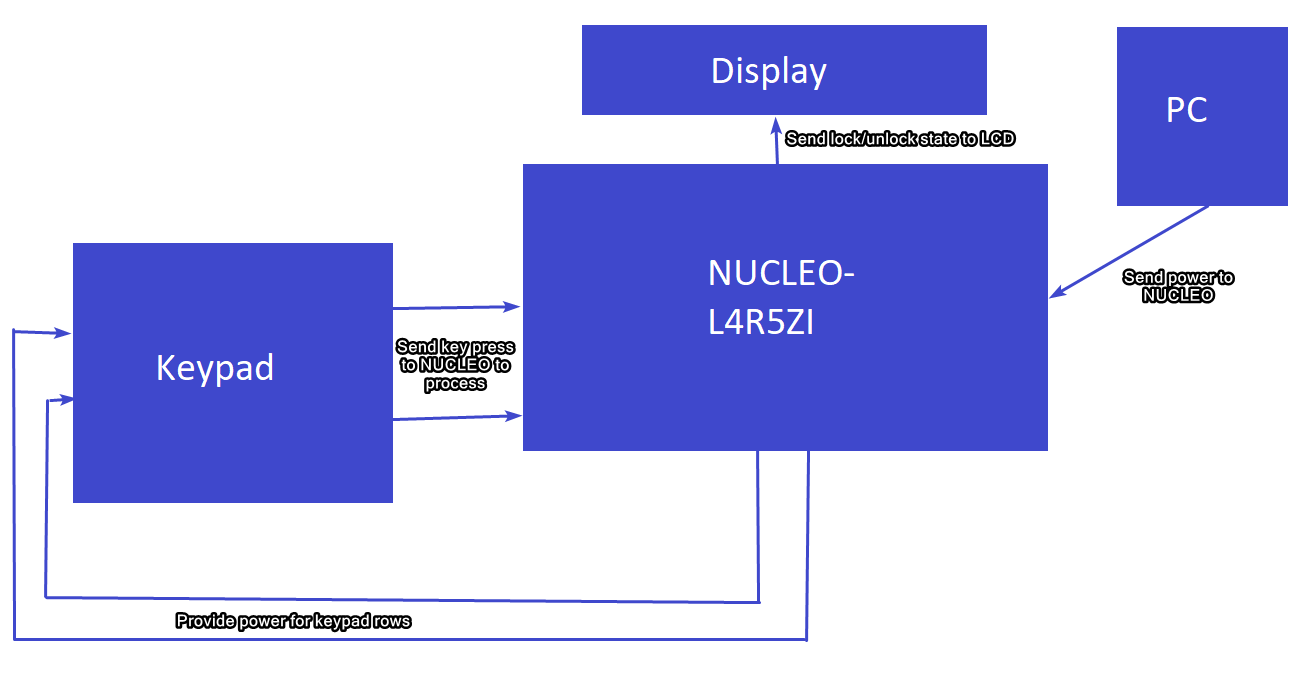
\includegraphics[width=\linewidth]{Block Diagram}\\
	\href{https://i.imgur.com/veSohTk.png}{\underline{Click here}} for a zoom-in-able imgur version of this image.
	\pagebreak
	\section{Functionality Diagram}
	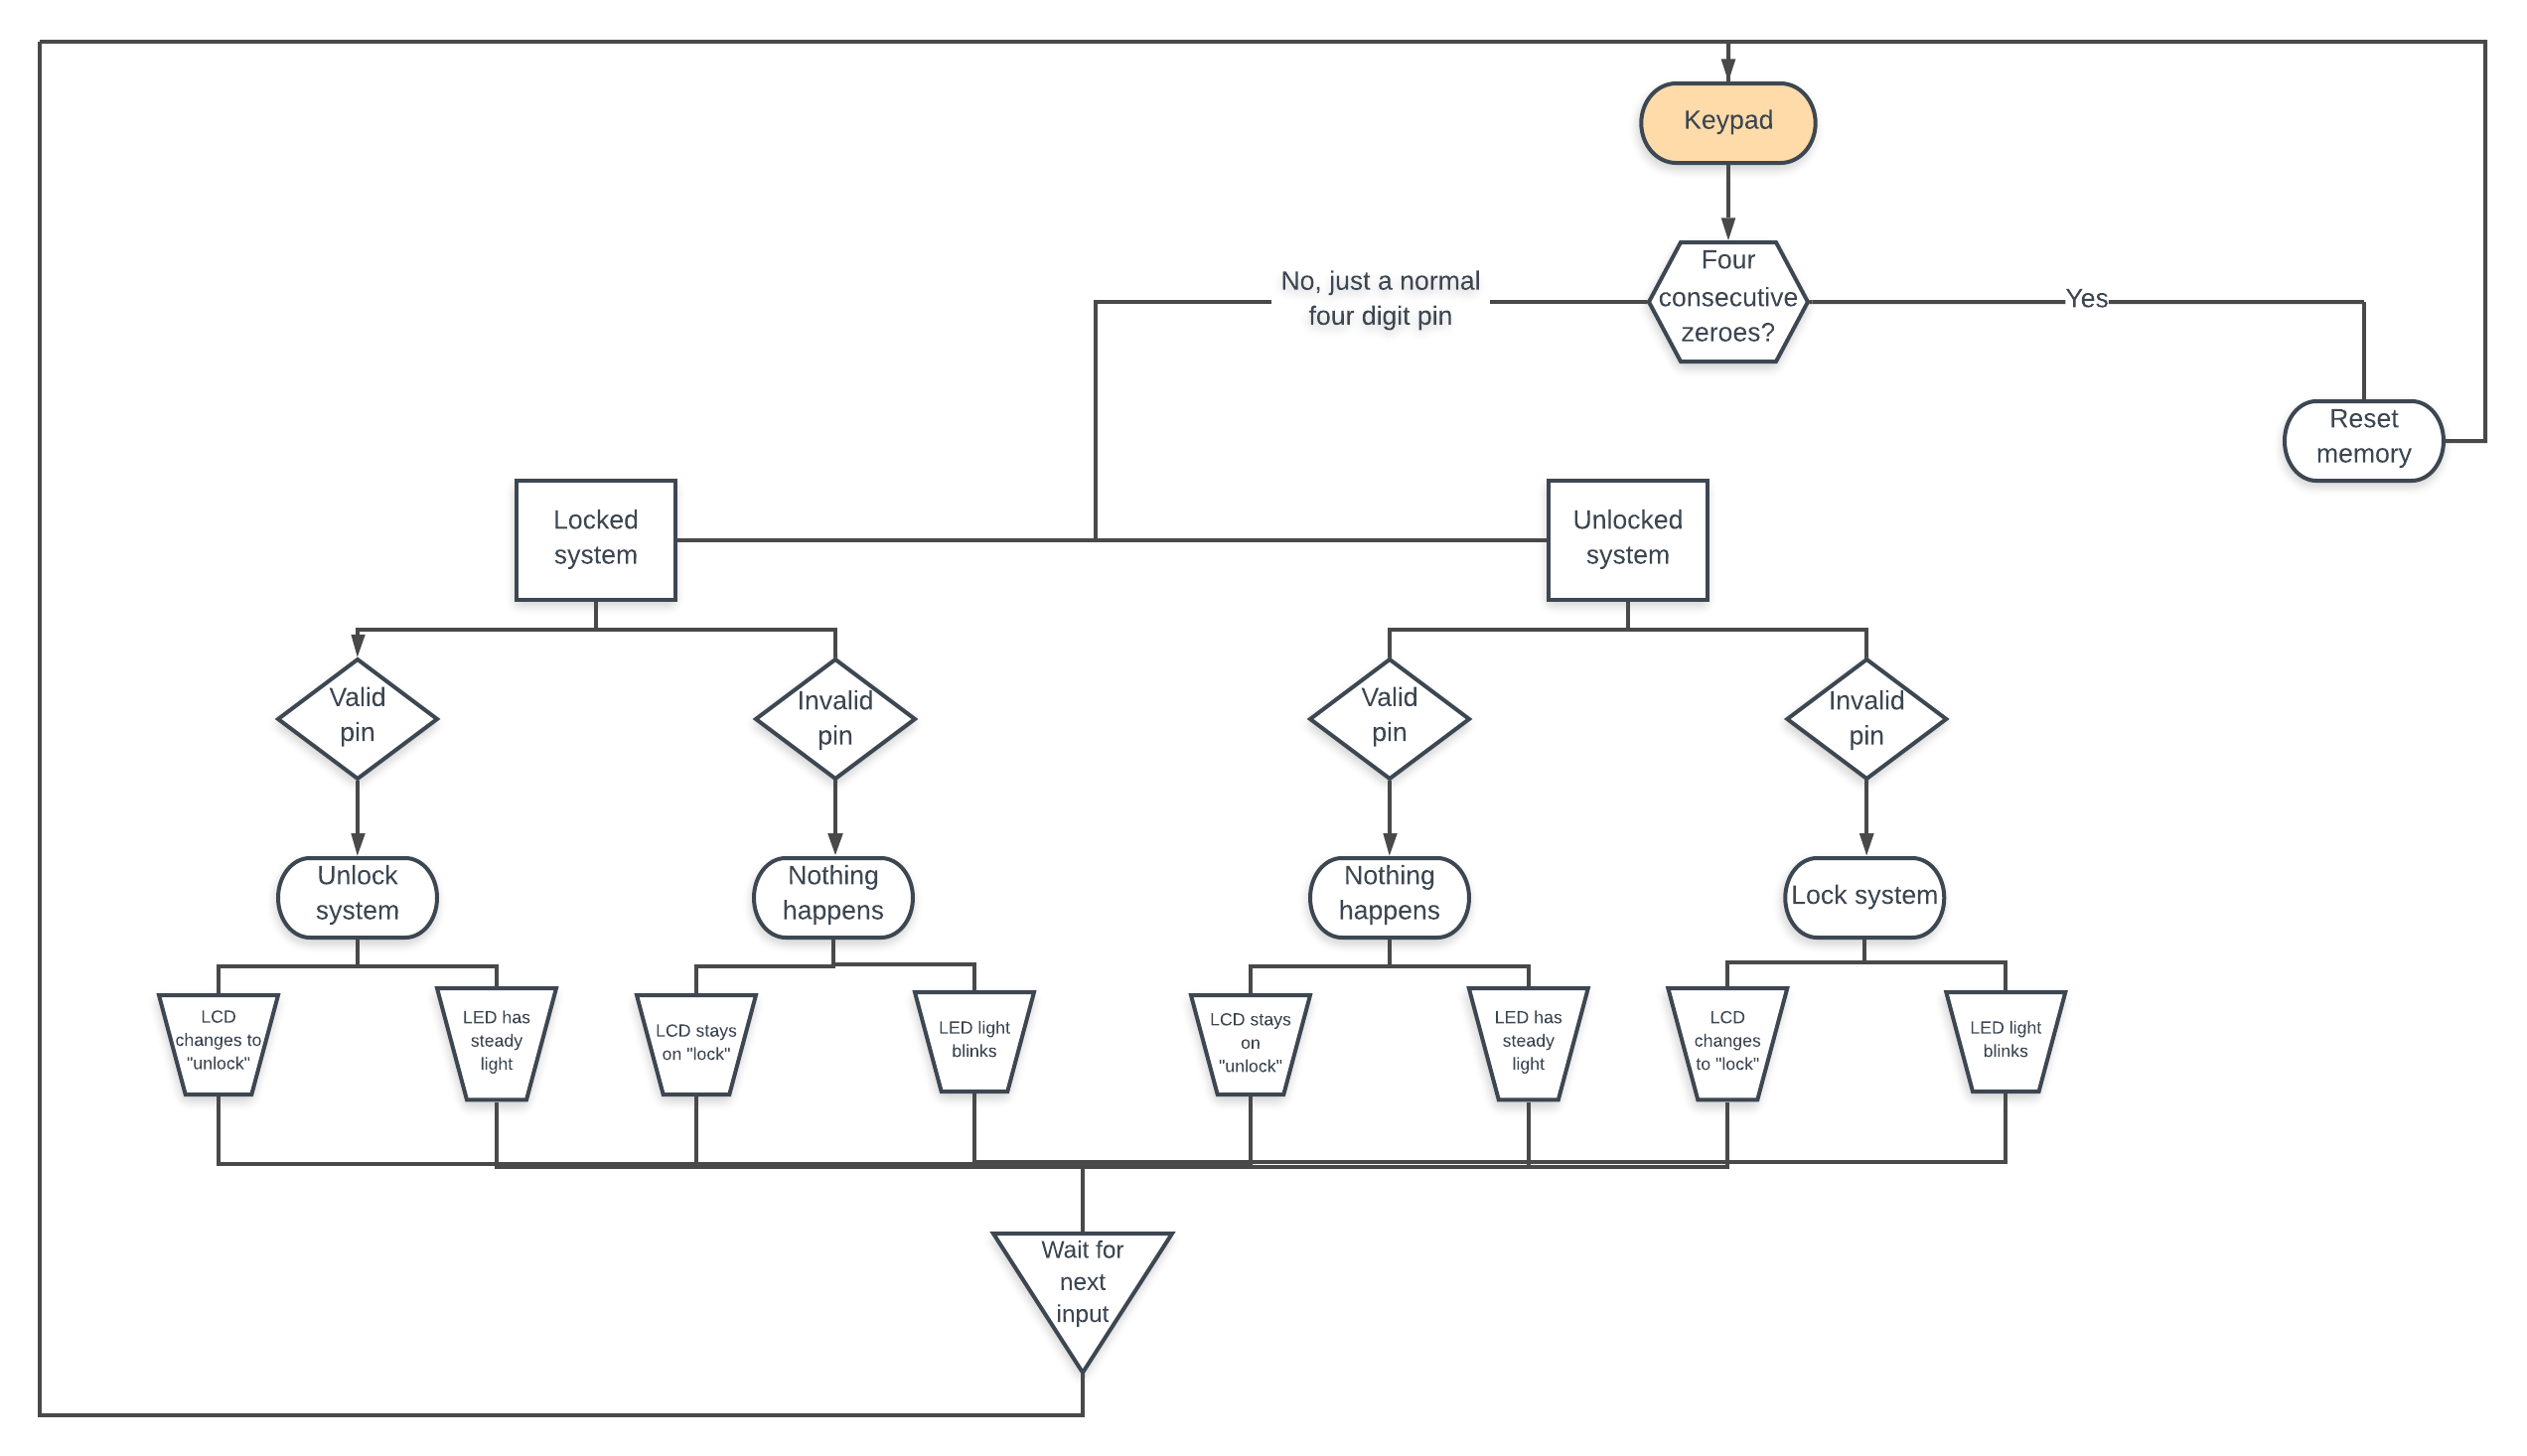
\includegraphics[width=\linewidth]{Flowchart}\\
	\href{https://i.imgur.com/dgIrW47.png}{\underline{Click here}} for a zoom-in-able imgur version of this image.
	\pagebreak
	\section{Bill of Materials}
	\begin{itemize}
		\item A Grove 16x2 LCD display
		\item A Nucleo-L4R5ZI
		\item A USB A to Micro-USB B cable
		\item A 4x4 matrix array keypad
		\item Jumper cables for connections
		\item Access to a desktop computer (software being used: \LaTeX{ }and MBed Studio)
	\end{itemize}
	\pagebreak
	\section{Schematic Diagram}
	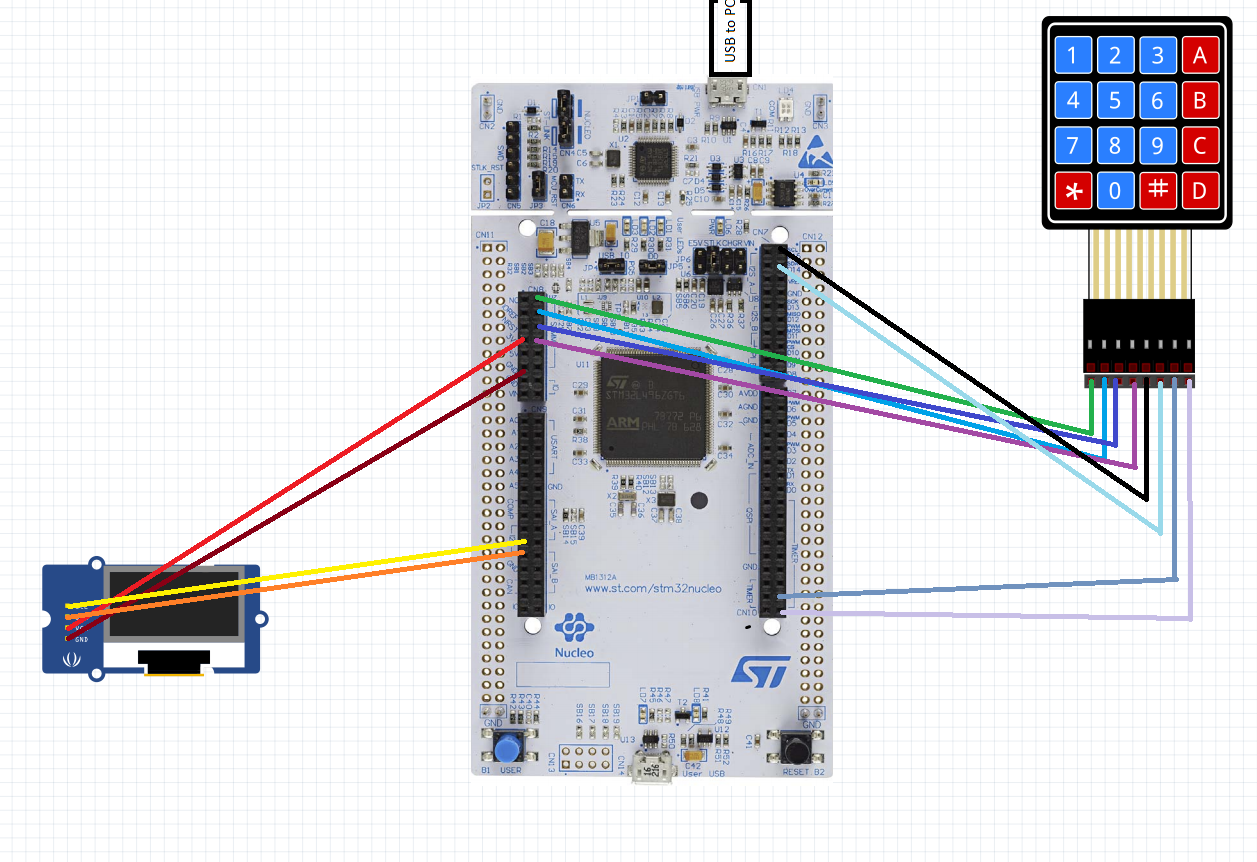
\includegraphics[width=\linewidth]{Schematic Diagram}\\
	\href{https://i.imgur.com/9wGSV8Q.png}{\underline{Click here}} for a zoom-in-able imgur version of this image.
	\pagebreak
	\section{Test Plan}
	The best way to test a system such as this is to go through all (in this case five) of the system's states and ensure they are functioning properly.
	
	The order of the tests described below assumes that the system began or is currently in a locked state. Additionally, the reset button should be pressed prior to testing to ensure that the memory is cleared. 
	\begin{enumerate}
		\item Since we had just pressed the reset button, it is most convenient to begin testing here. A password reset can be done at four points: 0/4 digits entered, 1 digit entered, 2 digits entered, and 3 digits entered. Since the memory gets reset after the fourth digit is processed, 0 digits entered and 4 digits entered are functionally identical. A test plan to test these four conditions is detailed below.
		\begin{itemize}
			\item 0/4 digits: At this state, the reset button shouldn't do anything. A pass for this test would be the system not crashing. 
			\item 1 digit: Enter numbers in this order: 9-A-4-0-7. If this is recognized as an incomplete input, the test has been passed. For an incomplete input, there should be no feedback from the system for as far as it is aware, only three values have been provided. 
			\item 2 digits: Enter numbers in this order: 9-4-A-0-7. Similarly to the single digit test case, if this is recognized as an incomplete input the test has been passed.
			\item 3 digits: Enter numbers in this order: 9-4-0-A-7. Once again, if this is recognized as an incomplete input the test has been passed.
		\end{itemize}
		\item Next, we should test that the system remains locked with an invalid input. Since the system should remained locked if provided any one of 9,999 different combinations, a couple different pins should be tested for thoroughness. Some good values to test are: 9406, 9408, 0000, 9999, 2994, 9542, and 5826. The reasoning behind each of these is below. All seven of these numbers should \textit{fail}. If they do, you can move on to the next test. 
		\begin{itemize}
			\item 9406 and 9408 are respectively the integers one smaller and one larger than the correct input. This tests to ensure that the system doesn't check for a \textit{range} of correct values, but is rather looking for a singular specific input. 
			\item 0000 and 9999 are respectively the smallest and largest inputs possible given four numbers. This ensures that both small and large numbers can fail.
			\item 2994, 9542, and 5826 are three randomly generated numbers and just serve to enlarge the sample size.
		\end{itemize}
		\item Afterwards, we should test if the system can unlock safely. This test is quite easy to undertake; just input 9407. If the system correctly unlocks, you may move on to the next test. 
		\item The system should now be unlocked. For the next test, input the correct input (9407) once again. If nothing happens (besides the LED indicating a correct input), the system is functioning correctly, and you may move on to the next test.
		\item Finally, we should test that an unlocked system can lock correctly when provided an invalid input. Similarly to the second test, for thoroughness it is wise to test a wide range of values. Some good values to test are: 9406, 9408, 0000, 9999, 6441, 8583, and 3427. The reasoning for these values is identical to those from the first test. 
	\end{enumerate}~\\
	Should all of these test be passed, the system has passed inspection and works completely as requested.
\end{document}